\begin{figure}[H]
    \centering
         \centering
         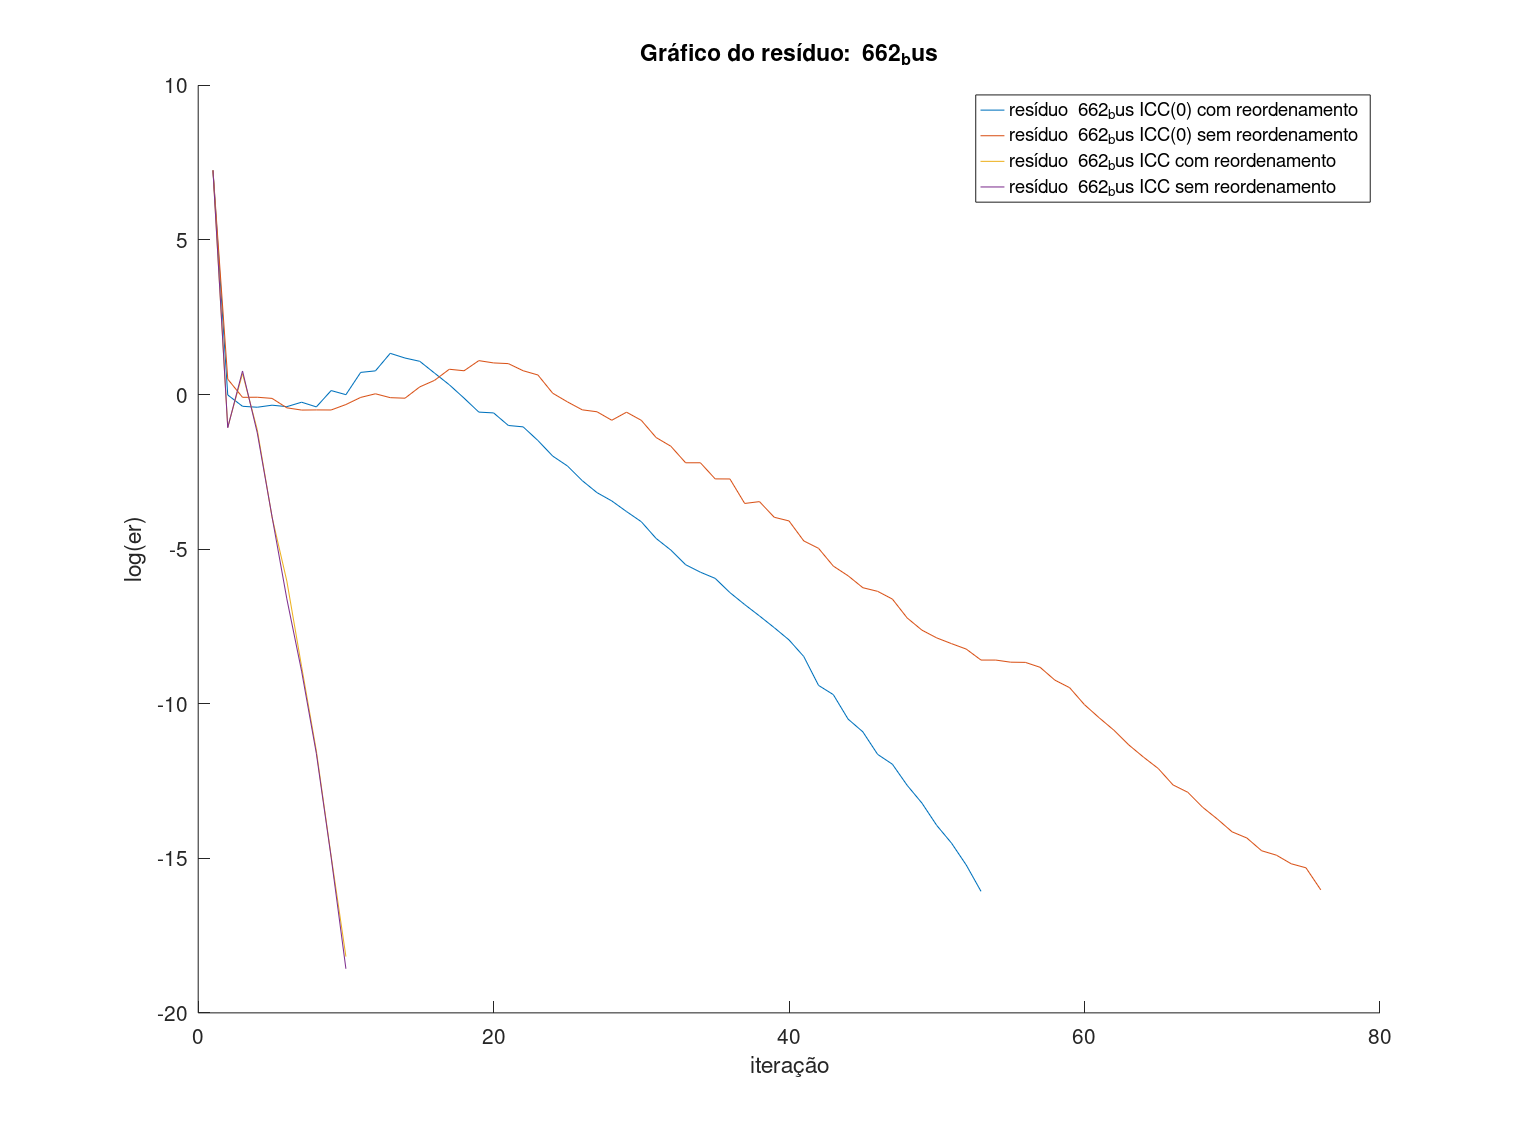
\includegraphics[width=.6\linewidth]{images/662_bus.png}
         \caption{Gráfico do Resíduo da matriz \textit{662\_bus}}
         \label{fig:bus-res}
\end{figure}

\begin{figure}[H]
    \centering
         \centering
         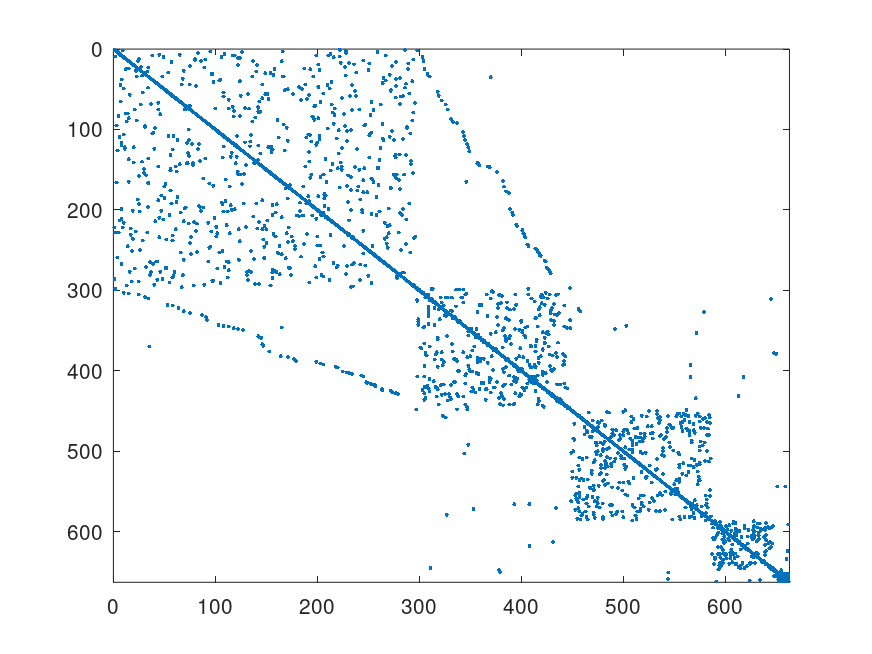
\includegraphics[width=.5\linewidth]{images/662_bus_spyA.png}
         \caption{Spy de da matriz \textit{662\_bus}}
         \label{fig:bus-spy-a}
\end{figure}

\begin{figure}[H]
    \centering
    \begin{subfigure}[t]{0.4\linewidth}
         \centering
         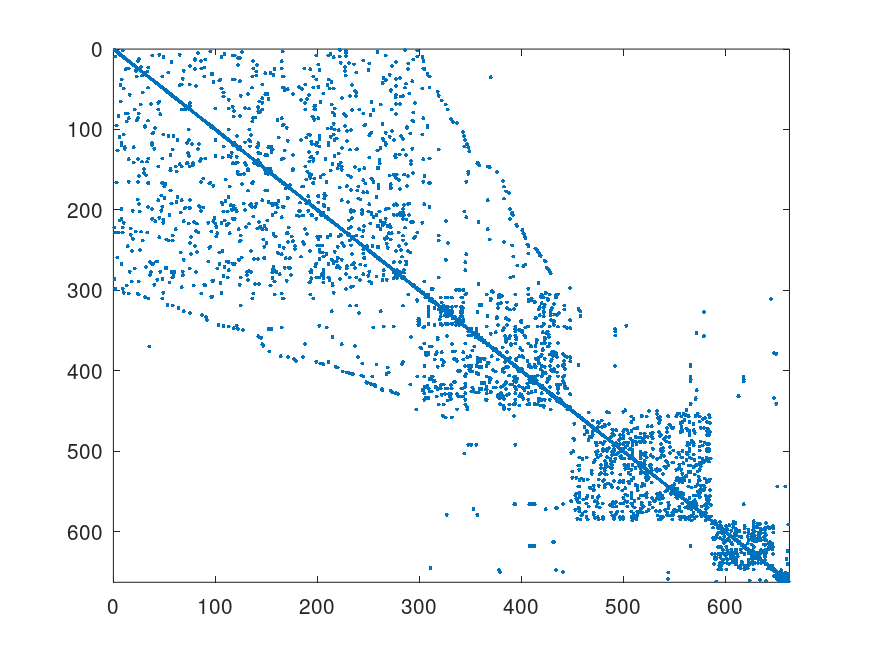
\includegraphics[width=\textwidth]{images/662_bus_spyM_ICC(0)_sem.png}
         \caption{Spy após ICC(0) sem reordenamento}
         \label{fig:bus-icc0-sem}
    \end{subfigure}
    \quad
    \begin{subfigure}[t]{0.4\linewidth}
         \centering
         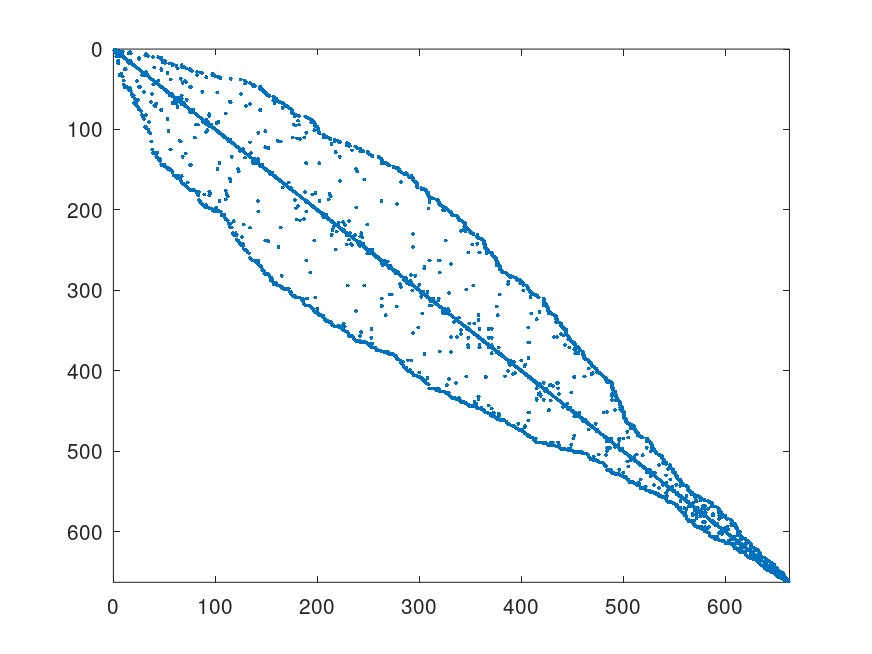
\includegraphics[width=\textwidth]{images/662_bus_spyM_ICC(0)_com.png}
         \caption{Spy após ICC(0) com reordenamento}
         \label{fig:bus-icc0-com}
    \end{subfigure}
    \par\bigskip
    \begin{subfigure}[t]{0.4\linewidth}
         \centering
         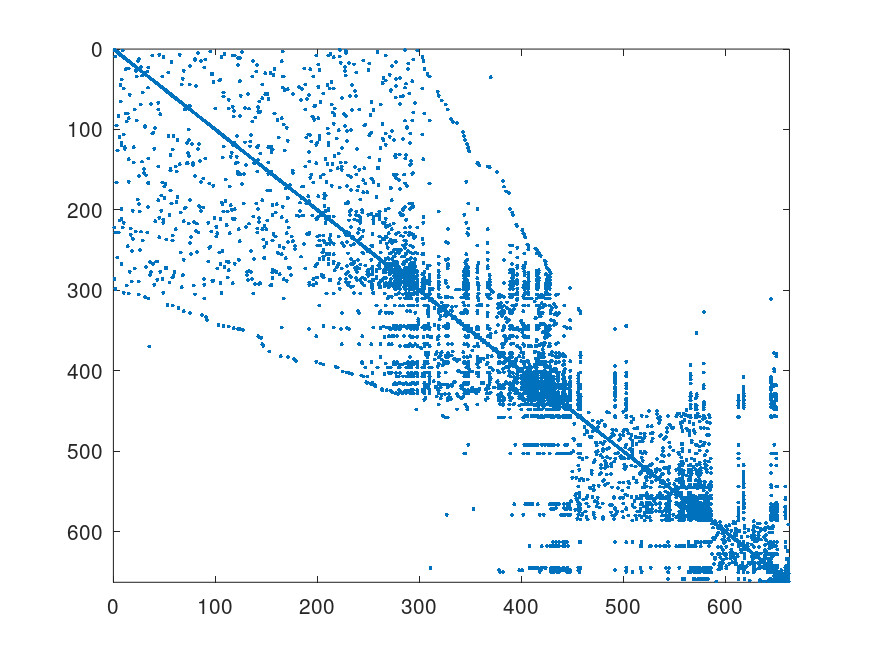
\includegraphics[width=\textwidth]{images/662_bus_spyM_ICC_sem.png}
         \caption{Spy após ICC sem reordenamento}
         \label{fig:bus-icc-s}
    \end{subfigure}
    \quad
    \begin{subfigure}[t]{0.4\linewidth}
         \centering
         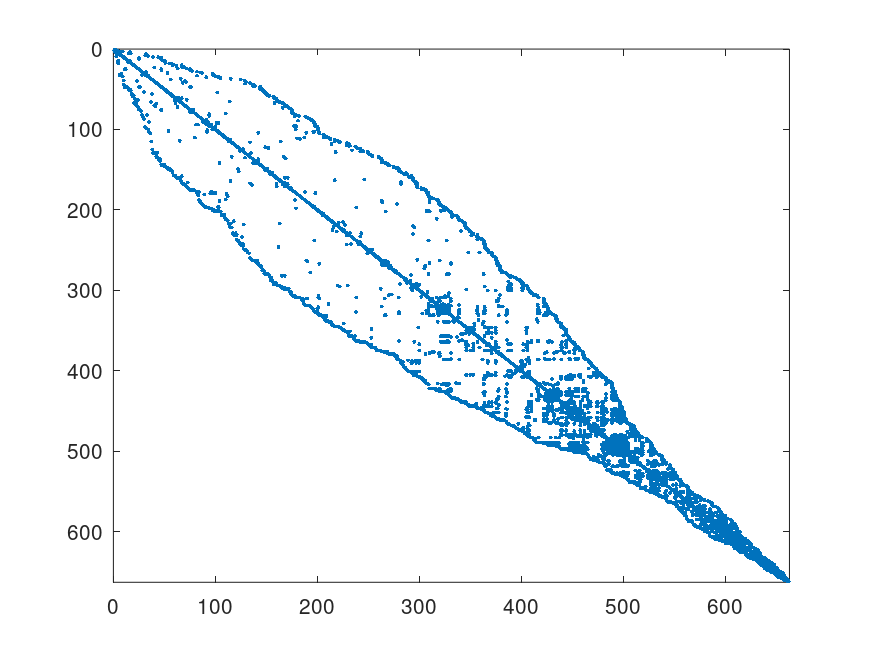
\includegraphics[width=\textwidth]{images/662_bus_spyM_ICC_com.png}
         \caption{Spy após ICC com reordenamento}
         \label{fig:bus-icc-c}
    \end{subfigure}
    \caption{Gráficos do preenchimento de \textit{662\_bus}.}
    \label{fig:bus}
\end{figure}